\documentclass[../thesis.tex]{subfiles}
\begin{document}
\chapter{appendix}

\section{model implementation}

In this part the model implementation and execution is explained.

When having to run a model for a variety of sets of input values it is useful to think about reducing the manual performed steps to a minimum. This has the advantages to provide a scalable solution if the set of input variables increases or the number of different values that need to be looked at grows. When having to set large amount of variables at different places within the model manually, the process is prone to errors that might not be detected until the results are computed or in case of small ones are not detected at all.

In general the developed solution follows the guideline shown in \autoref{fig: software_guideline}.

\begin{figure}[htbp]
	\centering
	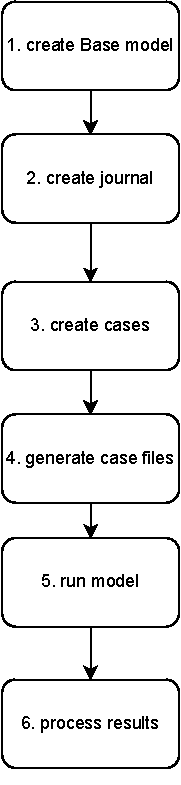
\includegraphics[scale=1.0]{software_proc}
	\caption{implementation guideline}
	\label{fig: software_guideline}
\end{figure}

The first step that needs to be done when creating a set of cases is the creation of a base model. This step mostly includes the geometry creation and meshing. It is important that the results exported, that are directly influenced by the mesh are able to be further processed. That is why the mesh in this work's base models mostly consists out of squares and rectangles. The creation of the base model is done using the tool \texttt{ANSYS WORKBENCH}.

The next step is to create a journal that sets all the values for the input variables. The file is called journal according to \cite{manual2009ansys} and is used to automate \texttt{ANSYS FLUENT} model execution. This journal can easily be created by using the build in macro recording tool of \texttt{ANSYS FLUENT}. Within this journal all needed settings that are not already set within the base model itself must be included. A part of such a journal is shown in \autoref{lst: journal}. One of the last steps of such a journal is the export of a model and a data file to a target location chosen by the user. This step is needed when looking into parallel execution of models that will be explained later.

%\lstinputlisting[language=Bash, caption=journal example]{code/testjournal.jou} 
%\lstinputlisting[caption=journal example, label=lst: journal]{code/testjournal.jou}

\definecolor{codehighlight}{rgb}{0.95,0.8,0.8}
\lstinputlisting[caption=journal example, label=lst: journal, basicstyle=\fontsize{9}{10}\selectfont\ttfamily, linebackgroundcolor={%
	\ifnum\value{lstnumber}=3\color{yellow!40}\fi 
	\ifnum\value{lstnumber}=7\color{yellow!40}\fi    
	\ifnum\value{lstnumber}=8\color{yellow!40}\fi
	\ifnum\value{lstnumber}=13\color{yellow!40}\fi
}
]{code/testjournal.jou}

From the highlighted lines in \autoref{lst: journal} it can be seen that for each variable that needs to be set by the journal a variable name is defined and put between to two \% signs for easier identification. With this approach new variables can be efficiently added. When the journal is created by the user and the journal functionality is tested and proven the cases need to be created. A case is defined here as one model execution with a set of input parameters and their values. The cases can be created in different ways but need to be provided in .json format in the end. An example of such a case in correct format can be seen in \autoref{lst: case}. The file providing the cases can contain as many as needed. 

\lstinputlisting[caption=case example, label=lst: case, basicstyle=\fontsize{9}{10}\selectfont\ttfamily]{code/testcase.json}

After the cases are provided and all previous steps are done as well all cases can be created by running the developed tool \texttt{journal.py}.
This tool creates a folder for each case at the destination provided within \texttt{conf.json} and creates all files needed to execute the case. This script needs to be run on a machine that has \texttt{ANSYS FLUENT} installed and is able to write to the desired destination. The version used here is \texttt{Fluent 2022 R1}. Having all files needed for case execution within the case's folder makes parallel case execution possible because cases have no cross referenced files. That also helps with developing, debugging and checking the case at future times, as all things necessary are there.

If all cases are created successfully they can be run in parallel on an High Performance Computing (HPC) Cluster. The journal template files developed within this work also provide a variant for local execution but that is not recommended when having a large amount of cases to run and if the number of cells get rather high. Since a HPC Cluster was used here this work focuses on that execution variant.

\begin{figure}[htbp]
	\centering
	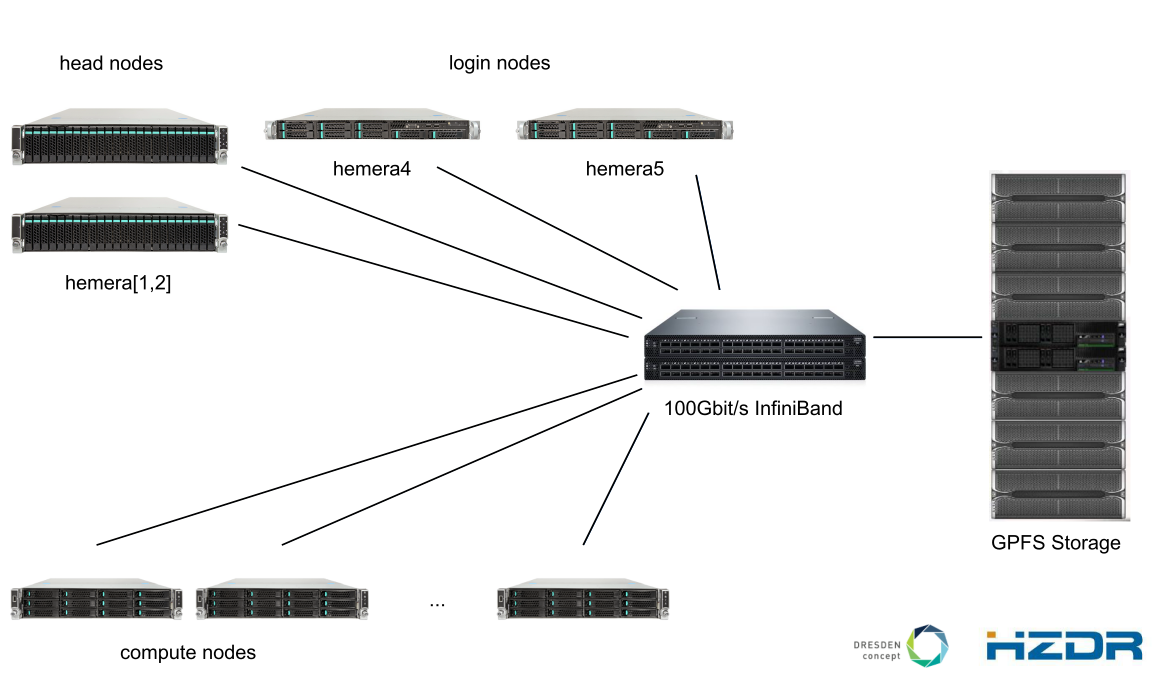
\includegraphics[scale=0.5]{HPC_Cluster}
	\caption{HPC Cluster Overview}
	\label{fig: HPC_Cluster}
\end{figure}

A brief overview of the Cluster used is provided in \autoref{fig: HPC_Cluster} \cite{schulz2022hardware_and_num}. A Cluster usually consists of 5 different components. To provide a high amount of computational power compute nodes are needed. This can be as many as rack space and or other limiting factors are available. To feed the compute nodes with calculations to perform the head nodes are doing the load balancing. A task that needs to be performed on the cluster is called job. These jobs are created on the login nodes and then submitted to the head nodes that run a queueing system. The one used here is \texttt{slurm}. For data and storage access all nodes are connected to a storage server using an industry standard high capacity network connection. It is not wise to run the login and head nodes on the same piece of hardware as one could think because if the head nodes crash the hole cluster becomes inoperable. To minimise this risk these two tasks are separated onto different machines.

For the queueing system \texttt{slurm} to accept a job a few parameters need to be set. Each job needs to have a partition and wall time set. The partition refers to a given queue on the cluster. There are different queues for different purposes and not all of them are available to each user.
The wall time is needed to set the maximum time a job is allowed to run. This prevents failing jobs to block the cluster for an infinite time. In addition to these two parameters, as shown in \autoref{lst: case} the hardware requirements of a job need to be set. This is the amount of nodes the job needs and the amount of CPUs that are reserved on each node. Since \texttt{ANSYS FLUENT} calculations can not be distributed over more than one node the amount of nodes is always 1. The CPU Cores used can be in a range of 1 to the maximum the hardware bound to the chosen queue has to offer. Higher demand of resources in combination with long wall times might lead to high queueing times so it is worth spending a thought on them. When having cluster access the developed script \texttt{run.sh} can be run with the option \texttt{-a} to run all jobs that have not generated any data. After some time has passed the script \texttt{time\_estat.py} can be run to get a estimation of the remaining job runtime using \autoref{eqn: rem_runtime}. The script will also warn the user if the set wall time is lower than the estimated execution time. The tool grabs the current job execution status out of the simulation's log file and uses the current job run time to calculate the total and remaining execution time. 
\begin{equation}
\label{eqn: rem_runtime}
t_{exec,remain} = \underbrace{\dfrac{t_{sim,total}}{t_{sim,current}} \cdot t_{exec,current}}_{\text{total execution time}}  - t_{exec,current} 
\end{equation}
These values can be easily compared with the set wall time.

\section{front positions}

Here you can see the front position plots for the cases with a gap height of 0.4mm in \autoref{fig: front_pos_h4_Sc2430} and \autoref{fig: front_pos_h4_Sc12000} and 0.6mm in \autoref{fig: front_pos_h6_Sc12000} and \autoref{fig: front_pos_h6_Sc2430}.

\begin{figure}[htbp]
	\centering
	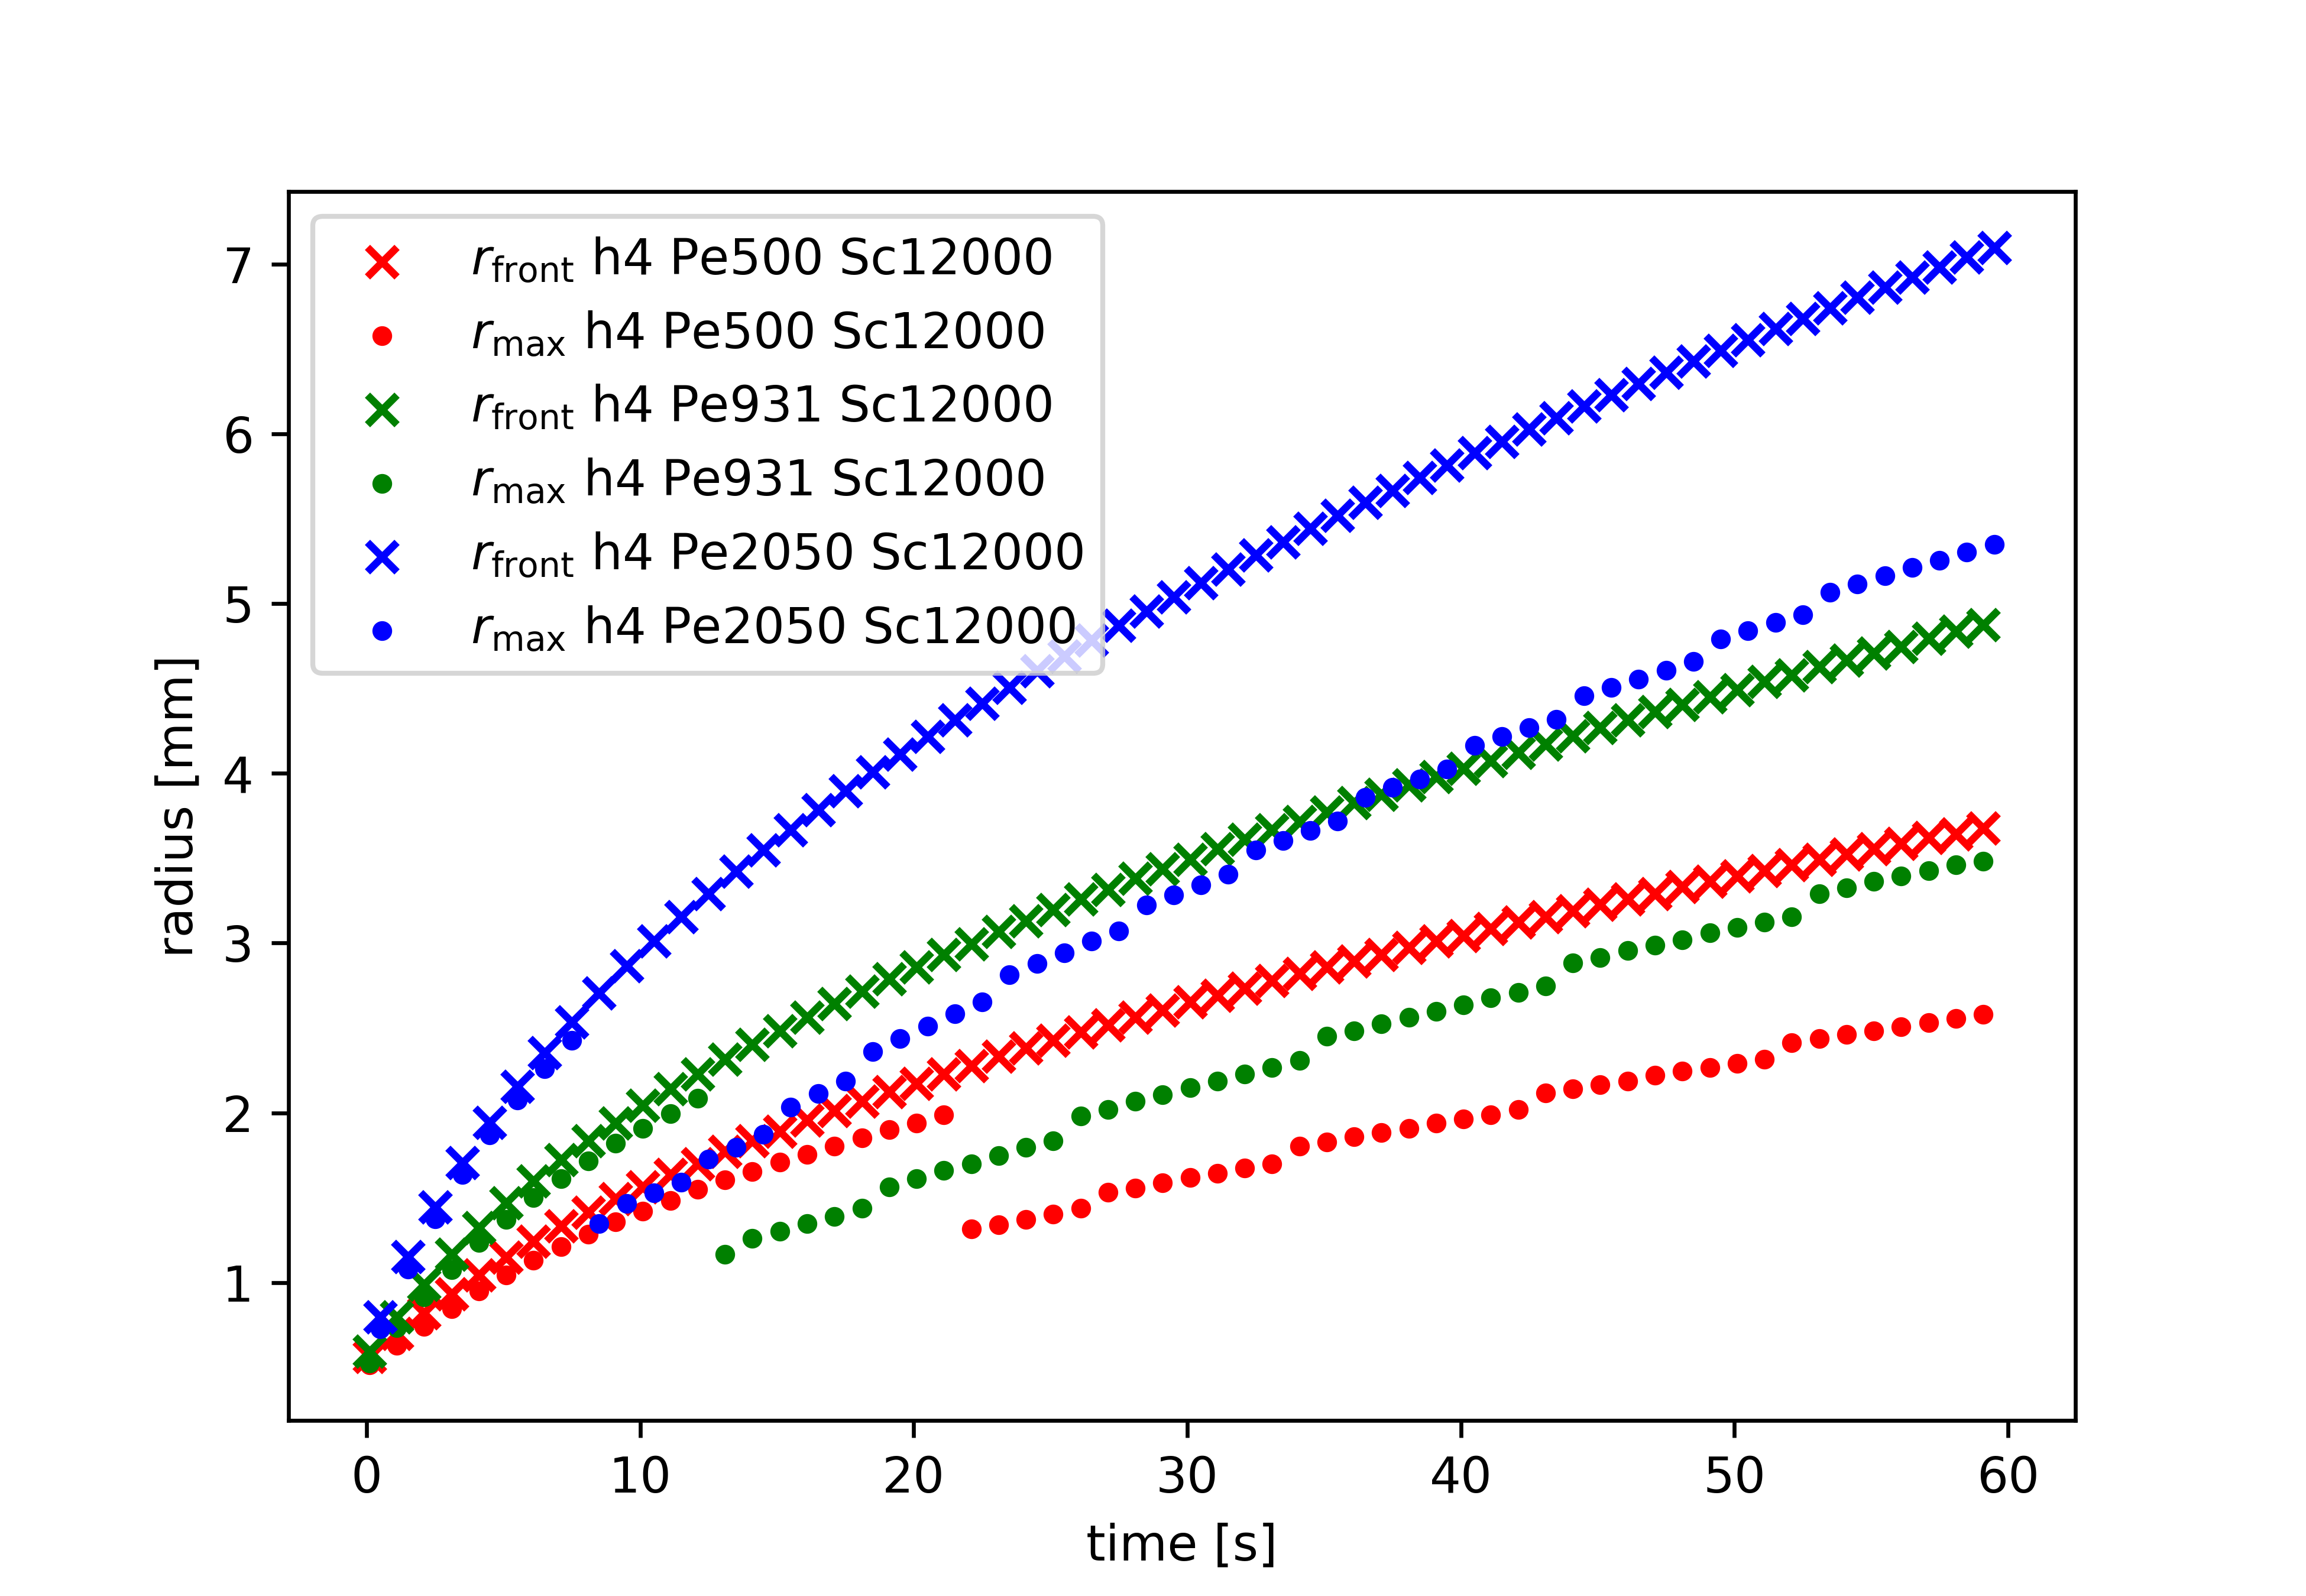
\includegraphics[width=.9\linewidth]{front_pos_h4_Sc12000}
	\caption{front positions for h0.4mm Sc12000\label{fig: front_pos_h4_Sc12000}}\bigskip
	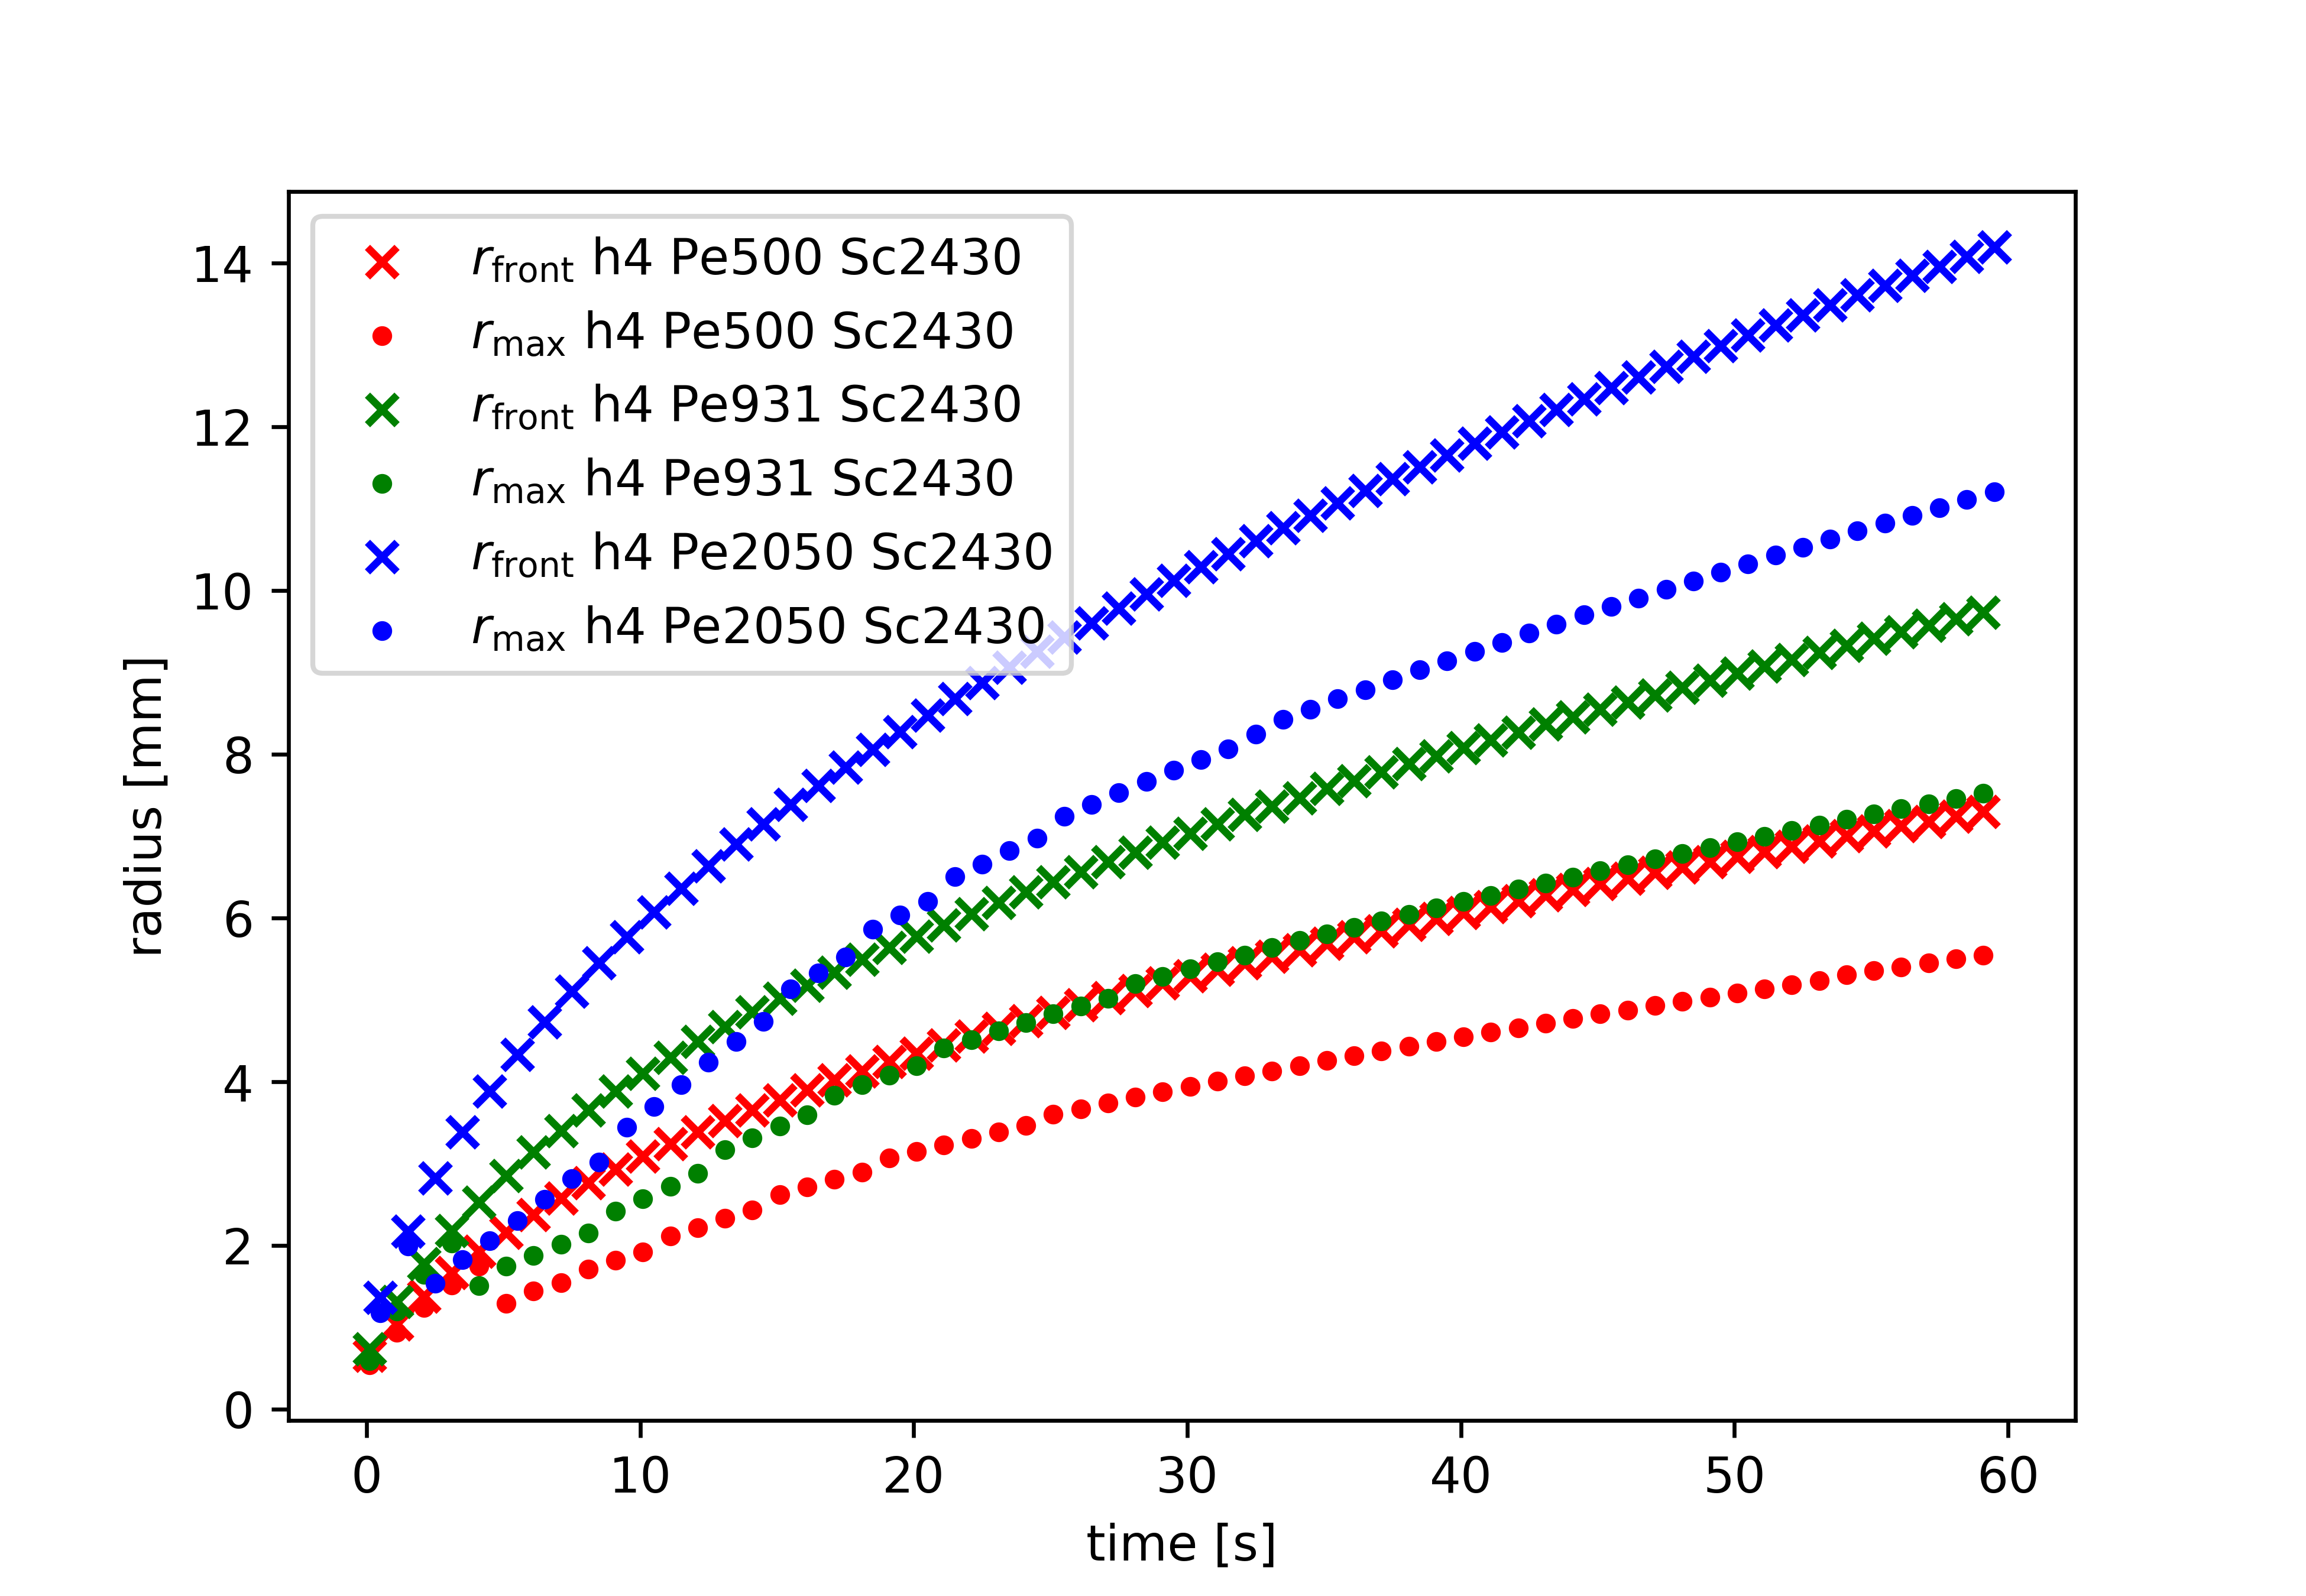
\includegraphics[width=.9\linewidth]{front_pos_h4_Sc2430}
	\caption{front positions for h0.4mm Sc2430\label{fig: front_pos_h4_Sc2430}}
\end{figure}

\begin{figure}[htbp]
	\centering
	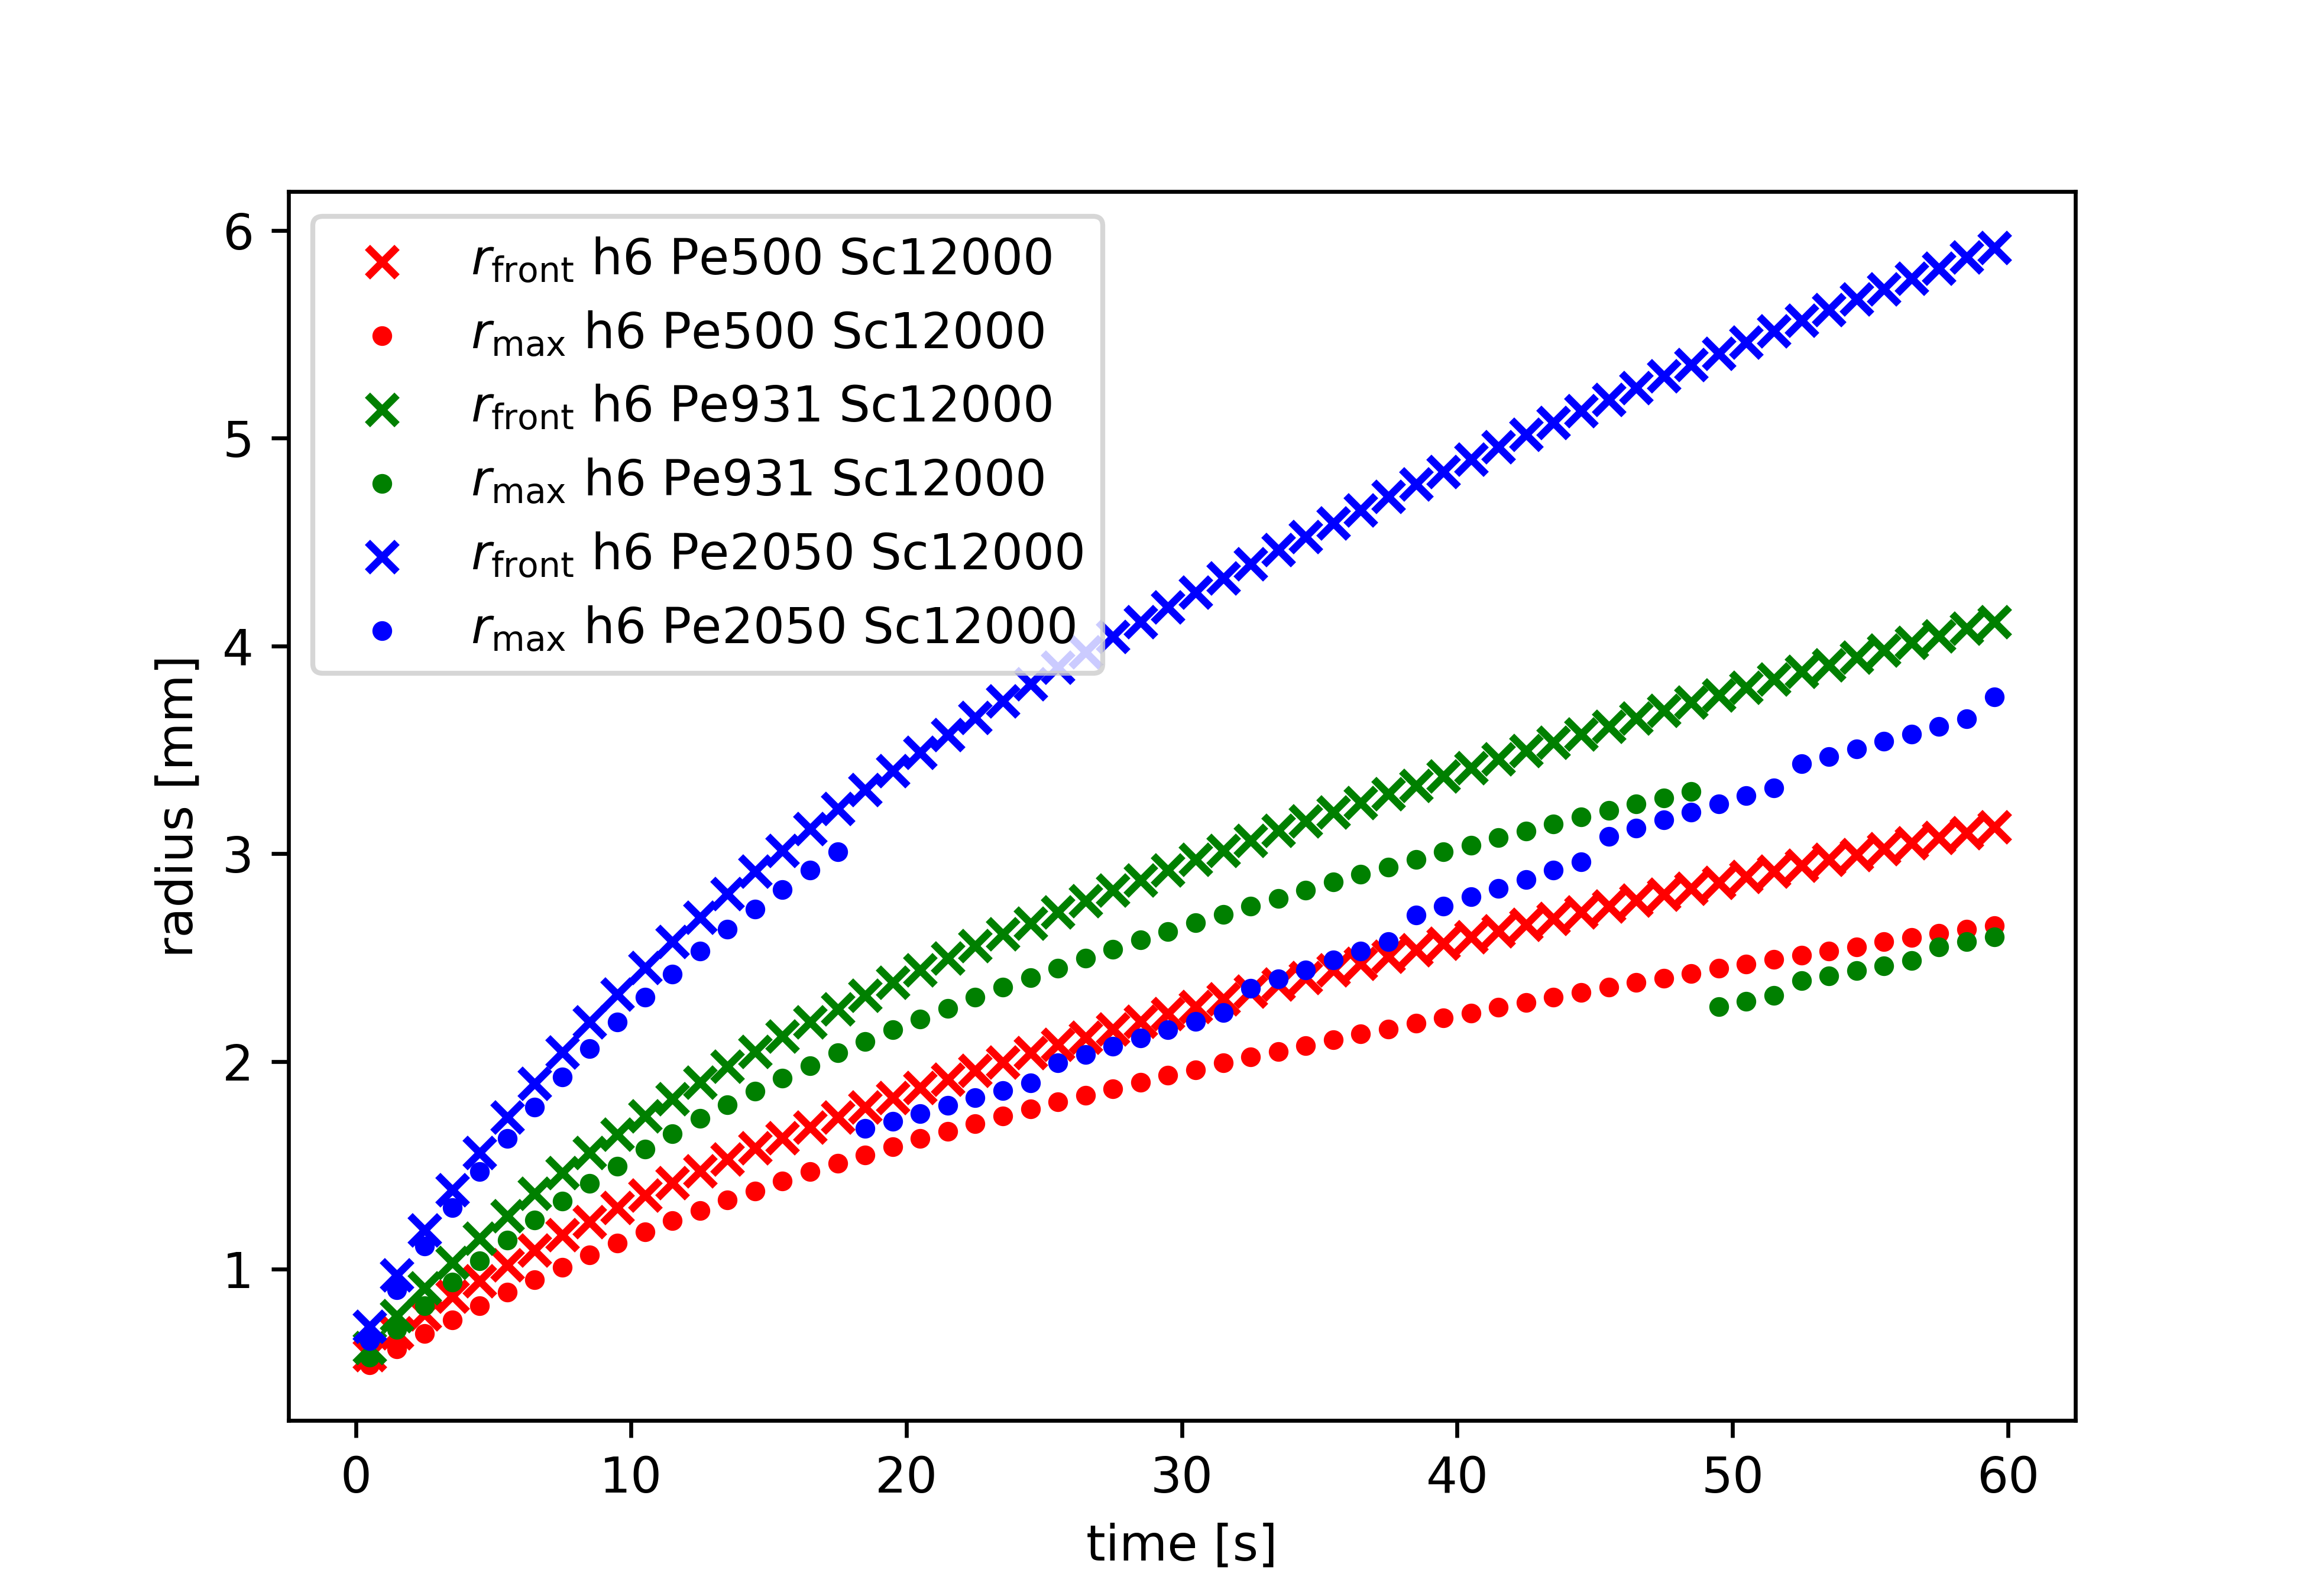
\includegraphics[width=.9\linewidth]{front_pos_h6_Sc12000}
	\caption{front positions for h0.6mm Sc12000\label{fig: front_pos_h6_Sc12000}}\bigskip
	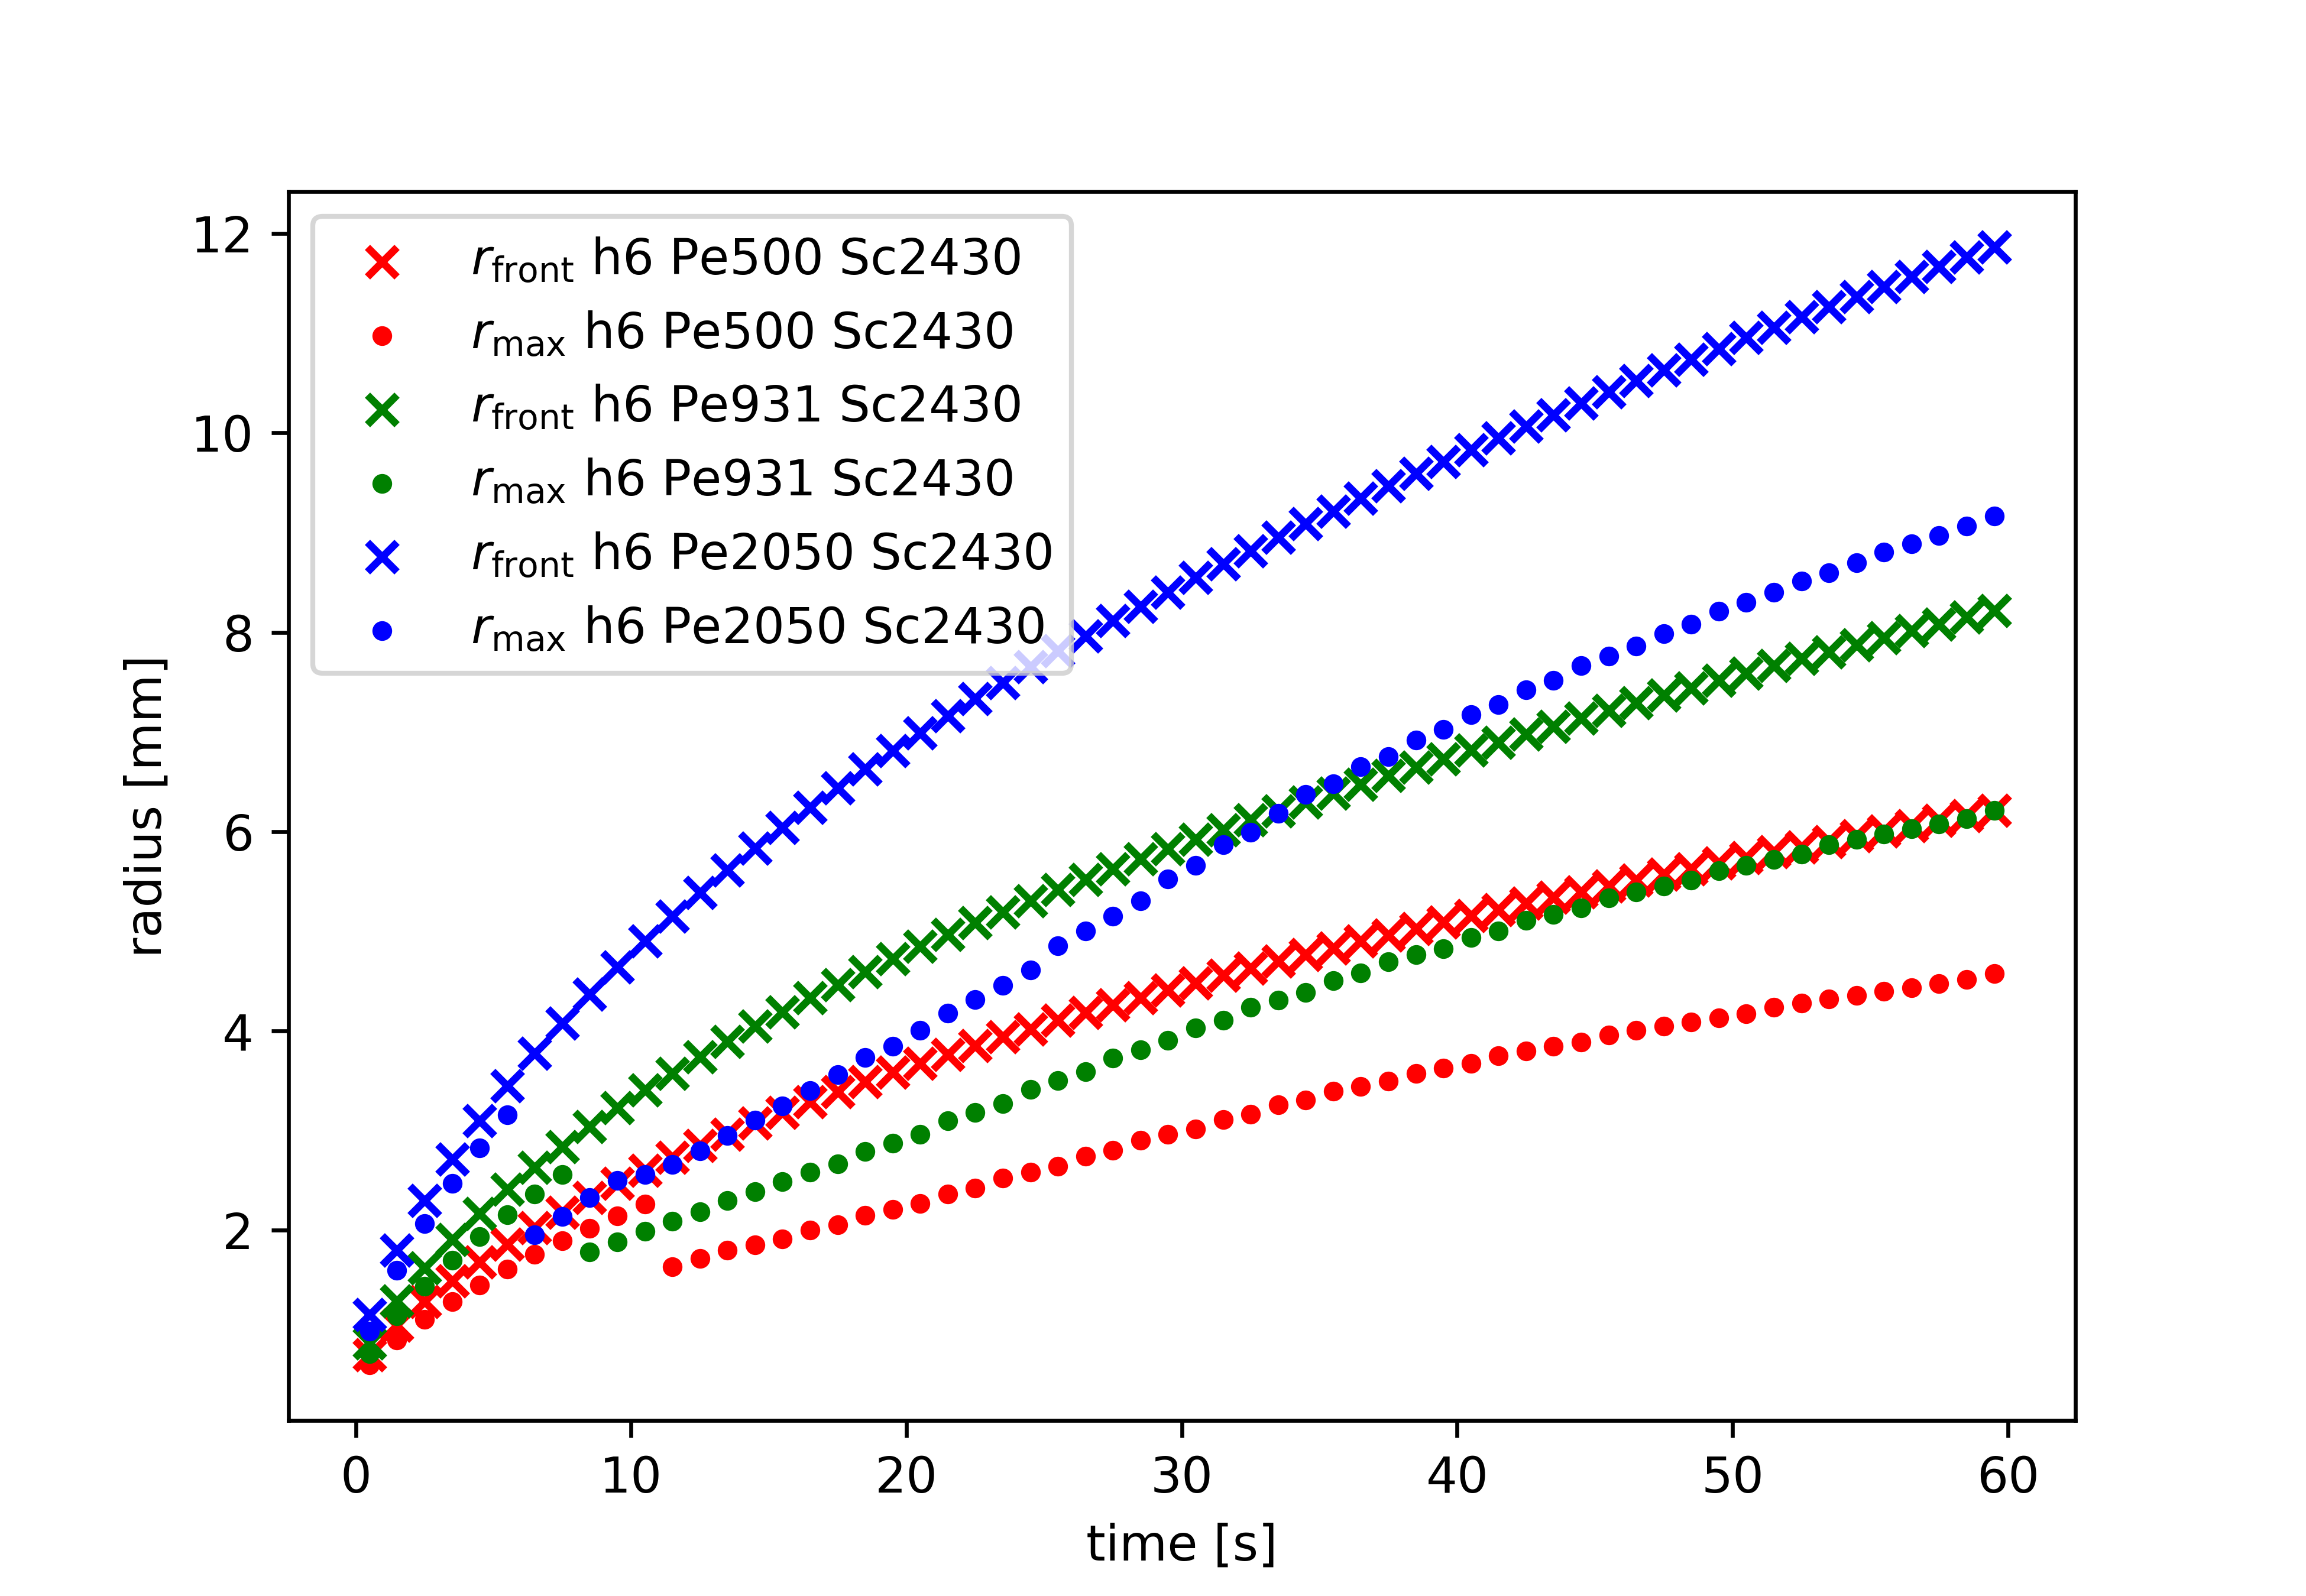
\includegraphics[width=.9\linewidth]{front_pos_h6_Sc2430}
	\caption{front positions for h0.6mm Sc2430\label{fig: front_pos_h6_Sc2430}}
\end{figure}

\end{document}